\section{角关联、偏振和$\delta$反演}\label{sec:5-7}

在建立原子核能级纲图（第~5.6~节）之后，确定各能级的自旋宇称 $I^\pi$、鉴别电磁辐射的多极阶数（偶极 $L=1$ 或四极 $L=2$）以及提取电四极/磁偶极振幅混合比 $\delta(E2/M1)$，构成了在束 $\gamma$ 谱学向微观核结构模型（如转子模型、粒子-转子耦合与手征/摆动动力学）过渡的核心纽带。单纯的 $\gamma$ 跃迁能量与符合连接仅能提供能级拓扑连通性，无法独立锁定量子态的角动量与宇称。

在束重离子反应在自旋排列方向上具有天然的各向异性（见第~5.1~节）。出射 $\gamma$ 射线的空间角分布、双探测器方向角关联（DCO）以及康普顿线偏振度，携带着辐射场多极性与跃迁几率振幅干涉相位的直接信息。然而，由宏观角分布与偏振反演微观多极混合比 $\delta$ 是一类典型的非线性反问题。若对相位约定、退取向衰减、门选条件以及二次有理方程的多解特性缺乏严格界定，极易在谱学推断中产生两类典型偏差：其一，将特定几何下的 DCO 比值经验数值（如 1.0 或 0.5）当成普遍适用的多极性分界线，忽略门跃迁多极性与自旋序列的调制；其二，在角分布方程存在两个相容数学根时，依据理论模型的偏好人为舍弃其中一个物理自洽解分支，将理论假设冒充为独立实验判决。本节从统计取向张量与角分布几何展开出发，严格定义实多极混合比 $\delta$ 的相位约定，推导条件 DCO 强度比与康普顿散射偏振度方程，建立似然剖面下的双根反演与多解仲裁准则。

\subsection{角动量取向、辐射场几何与角分布理论}\label{subsec:5-7-1}

在束重离子完全熔合蒸发反应中，由于入射相对运动轨道角动量强烈偏向于垂直于束流轴的平面，初始复合核的磁子能级呈现高度取向的不均匀分布。在经历了相继的轻核子蒸发与统计非共振 $\gamma$ 级联后，待测母能级 $|i\rangle$（自旋为 $I_i$）可以保留一定程度的、沿束流轴（定为量子化 $z$ 轴）的轴对称取向。

母态的自旋取向状态由统计取向张量（Orientation Tensor）$B_k(I_i)$ 描述（Hamilton 1975 经典专著规范~\cite{book-hamilton-electromagnetic-interaction}）：
\begin{equation}\label{eq:5-7-bk-def}
B_k(I_i) \equiv \sqrt{2I_i + 1} \sum_{M_i} (-1)^{I_i - M_i} \langle I_i M_i I_i (-M_i) \mid k 0 \rangle P(M_i),
\end{equation}
其中 $P(M_i)$ 为磁子能级 $M_i$ 的统计布居几率，且满足归一条件 $\sum_{M_i} P(M_i) = 1$。由 Clebsch-Gordan 系数正交归一性，张量零阶项 $B_0(I_i) \equiv 1$ 对任意归一布居分布 $P(M_i)$ 恒成立（并不限于各向同性分布）。式中 Clebsch-Gordan 系数的次序规定了统计张量的相位约定；与 Hamilton 式~(12.73) 的张量记号相比，按式~\eqref{eq:5-7-bk-def} 定义的奇阶分量满足 $B_k = (-1)^k B_k^{\mathrm{Hamilton}}$，偶阶分量严格相同。

沿束流轴的轴对称性保证方位角量子数 $q = 0$（无非对角取向张量）。在所选量子化基中，若磁子能级布居满足非定向排列（Alignment）对称性 $P(M_i) = P(-M_i)$，则奇阶取向张量严格为零（$B_{\mathrm{odd}} = 0$）；若存在非对称极化（Polarization, $P(M_i) \ne P(-M_i)$），奇阶张量（如 $B_1$）可以非零。必须强调，对具有确定宇称的核态之间的通常电磁单光子跃迁，未分析光子偏振时需对两个出射螺旋度（$\lambda = \pm 1$）求和，强度分布中的奇阶辐射参数因螺旋度求和而严格抵消，因此强度级数中的奇阶贡献恒为零，即使母态本身具有非零奇阶取向张量也是如此（Hamilton 式~(12.180)--(12.189)）。受出射辐射场多极阶数（$L, L' \le L_{\max}$）与态自旋的三角选择定则双重限制，张量阶数截断于 $k \le \min(2I_i, 2L_{\max})$；对于最高多极阶数为四极（$L_{\max}=2$）的情形，强度展开式最多仅包含偶阶项 $k = 0, 2, 4$。

若母态是由一条指定的、未被探测的前级级联退激至 $I_i$，前级未观测级联退取向在单一路径下由去取向因子 $U_k = \prod_m U_k(m)$ 描述：
\begin{equation}\label{eq:5-7-deorientation}
B_k(I_i) = B_k(J_{\mathrm{CN}}) \prod_m U_k(m),
\end{equation}
若存在多条可能馈入路径，则应依据各分支布居份额加权求和。特别注意：若后文已直接使用目标母态的统计取向张量 $B_k(I_i)$，则其已内含了所有上游未观测级联的退取向效应，绝不可在后续角分布或表观展开系数中再次重复乘以相同的 $U_k$。

从取向母态 $|i\rangle$ 退激至末态 $|f\rangle$（自旋 $I_f$）发射的单色 $\gamma$ 射线，其相对于束流轴夹角 $\theta$ 的相对角分布函数 $W(\theta)$ 展开为偶阶 Legendre 多项式序列：
\begin{equation}\label{eq:5-7-w-theta-general}
W(\theta) = \sum_{k=0, 2, 4} B_k(I_i) A_k(\delta) Q_k P_k(\cos\theta),
\end{equation}
其中：
\begin{itemize}
\item $P_k(\cos\theta)$ 为标准第 $k$ 阶 Legendre 多项式（$P_0 = 1$，$P_2 = \frac{1}{2}(3\cos^2\theta - 1)$，$P_4 = \frac{1}{8}(35\cos^4\theta - 30\cos^2\theta + 3)$）；
\item $Q_k$ 为探测器对源张开有限立体角引起的几何衰减因子（Finite Solid-Angle Correction Factor），定义为 $Q_k = \int w(\Omega) P_k(\cos\alpha) d\Omega / \int w(\Omega) d\Omega$。作为标量因子的简化表示仅在探测效率分布 $w(\Omega) \ge 0$ 绕探测器中心晶体对称轴轴对称时严格成立（一般非轴对称几何须进行全立体角多极响应积分），满足 $Q_0 = 1$ 与 $|Q_k| \le 1$；
\item $A_k(\delta)$ 为由跃迁多极类型与多极混合比决定的辐射角分布系数；
\item 截断阶数 $k \le 4$ 建立在出射辐射场多极性不超过四极（$L, L' \le 2$）的基础之上（由选择定则 $k \le \min(2I_i, 2L_{\max})$ 严格限定）。
\end{itemize}
在实验数据分析中，角分布通常拟合为常规 Legendre 展开形式：
\begin{equation}\label{eq:5-7-w-theta-fit}
W(\theta) = 1 + a_2 P_2(\cos\theta) + a_4 P_4(\cos\theta),
\end{equation}
其中表观展开系数满足
\begin{equation}\label{eq:5-7-ak-apparent}
a_k = \frac{B_k(I_i) Q_k A_k(\delta)}{B_0(I_i) Q_0 A_0} = B_k(I_i) Q_k A_k(\delta),\qquad k=2,4,
\end{equation}
第二个等号采用了 $B_0(I_i) = Q_0 = A_0 = 1$ 的标准归一约定。此处 $B_k(I_i)$ 已直接表征待测态的实际取向度，式中绝无重复的 $U_k$ 因子。

\subsection{多极混合比$\delta$的相位约定与二次有理展开}\label{subsec:5-7-2}

当跃迁在角动量三角定则与宇称守恒下允许低阶辐射多极 $L$ 与高阶辐射多极 $L' = L + 1$ 同时存在时（最常见的是磁偶极 $M1$ 与电四极 $E2$ 竞争跃迁），出射场呈现多极相干叠加。

必须对实多极混合比 $\delta$ 给出严格的无量纲辐射几率振幅比定义。本节与第~5.9~节（式~\eqref{eq:5-9-delta-def}）及附录~A（式~\eqref{eq:appA-delta-def}）统一采用 Krane--Steffen（KS）多极混合比规范体系~\cite{lange-kumar-hamilton-1982-multipole-admixtures, book-hamilton-electromagnetic-interaction}：
\begin{equation}\label{eq:5-7-delta-def}
\delta(E2/M1) \equiv \frac{\gamma(E2)}{\gamma(M1)} = \frac{\sqrt{3}}{10} \frac{E_\gamma}{\hbar c} \frac{\langle I_f \| \mathcal{M}(E2) \| I_i \rangle}{\langle I_f \| \mathcal{M}_S(M1) \| I_i \rangle} = \frac{\sqrt{3}}{10} \frac{E_\gamma}{\hbar} \frac{\langle I_f \| \mathcal{M}(E2) \| I_i \rangle}{\langle I_f \| \mathcal{M}_\mu(M1) \| I_i \rangle}.
\end{equation}
在此定义下：
\begin{itemize}
\item $\delta$ 是出射光子场的电四极振幅与磁偶极振幅之比，是严格的无量纲纯数；
\item 它不是裸约化矩阵元的简单相比，而是内含了跃迁动量因子 $k_\gamma = E_\gamma / (\hbar c)$ 与相应的常数因子。当分母采用 SI 电荷型算符 $\mathcal{M}_S(M1) \equiv \mathcal{M}_\mu(M1) / c$ 时，其量纲为 $e\cdot\mathrm{fm}$，分子 $\mathcal{M}(E2)$ 量纲为 $e\cdot\mathrm{fm}^2$，动量因子 $E_\gamma/(\hbar c)$ 量纲为 $\mathrm{fm}^{-1}$，实现量纲严格对消；当分母采用磁矩型算符 $\mathcal{M}_\mu(M1)$（量纲 $\mu_N$）时，频率因子相应为 $E_\gamma/\hbar$，与第~5.9~节及附录~A 保持统一量纲与符号，避免无谓的单位重复折算；
\item 初末态波函数的全同规范位相在比值中精确对消，$\delta$ 的符号由跃迁算符定义与物理矩阵元内禀结构共同锁定。
\end{itemize}

在文献转换中，必须注意不同历史相位约定的映射关系：
除 Krane--Steffen（KS）约定外，核物理谱学还存在 Rose--Brink（RB）约定与 Biedenharn--Rose（BR）约定。在 Lange 等人~\cite{lange-kumar-hamilton-1982-multipole-admixtures} 给出的发射退激约定下，Krane--Steffen 约定与 Rose--Brink 约定的实数混合比相差一个负号：$\delta_{\mathrm{KS}} = -\delta_{\mathrm{RB}}$。\emph{若将文献中的 $\delta$ 符号转换至另一体系，必须同时将角分布干涉项系数的定义进行同步转换；绝不能在保留原公式几何系数形式的同时单独强行翻转 $\delta$ 的正负号}。

对于纯 $L$ 辐射与 $L'=L+1$ 辐射的混合，辐射角分布系数 $A_k(\delta)$ 可严格表征为混合比 $\delta$ 的二次有理函数~\cite{lange-kumar-hamilton-1982-multipole-admixtures}：
\begin{equation}\label{eq:5-7-ak-rational}
A_k(\delta) = \frac{F_k(L L I_f I_i) + 2\delta F_k(L L' I_f I_i) + \delta^2 F_k(L' L' I_f I_i)}{1 + \delta^2},
\end{equation}
其中 $F_k(L L' I_f I_i)$ 为纯几何性质的 Ferentz-Rosenzweig 系数（由 Racah 代数与 Wigner $6j$ 符号精确确定，其定义见Hamilton印539/PDF550式(12.168)）。对于最核心的 $M1+E2$ 跃迁（$L=1, L'=2$），式~\eqref{eq:5-7-ak-rational} 表达为：
\begin{equation}\label{eq:5-7-ak-m1e2}
A_k(\delta) = \frac{F_k(1 1 I_f I_i) + 2\delta F_k(1 2 I_f I_i) + \delta^2 F_k(2 2 I_f I_i)}{1 + \delta^2}.
\end{equation}
分子中的交叉项 $+2\delta F_k(1 2)$ 直观展示了电四极与磁偶极发射振幅之间的量子力学相干干涉。在 Hamilton 专著与 Lange 等人的公式体系中，该正干涉交叉项严格对应于 Krane--Steffen 约定，绝不可将其直接标为 Rose--Brink 公式。

\subsection{定向态方向角关联（DCO）与门谱几何修正}\label{subsec:5-7-3}

虽然一维角分布 $W(\theta)$ 理论优美，但在重离子在束实验中，直接测量单谱角分布往往受到靶核连续本底与杂质峰的严重干扰。在多探测器阵列中，更常用的实验方法是在二维符合矩阵（第~5.6~节）上建立\emph{定向态方向角关联}（Directional Correlation from Oriented States, DCO）。

考虑由级联跃迁 $\gamma_1$ 与 $\gamma_2$ 构成的符合事件。实验将探测器分别放置在特定的两个极角 $\theta_1$ 与 $\theta_2$（相对于束流轴，通常选取 $90^\circ$ 与前向/后向角度如 $30^\circ$ 或 $135^\circ$）。由非对称符合矩阵（见第~5.6~节的非对称矩阵定义）导出的实验 DCO 比值严格定义为条件门选强度之比：
\begin{equation}\label{eq:5-7-dco-def}
R_{\mathrm{DCO}} \equiv \frac{N_{\gamma 1, \gamma 2}(\theta_1, \theta_2)}{N_{\gamma 1, \gamma 2}(\theta_2, \theta_1)} \times \frac{\varepsilon_{\mathrm{p}}(\theta_2, E_{\gamma 1}) \varepsilon_{\mathrm{p}}(\theta_1, E_{\gamma 2})}{\varepsilon_{\mathrm{p}}(\theta_1, E_{\gamma 1}) \varepsilon_{\mathrm{p}}(\theta_2, E_{\gamma 2})},
\end{equation}
其中 $\varepsilon_{\mathrm{p}}(\theta, E)$ 为该角度通道的绝对全能峰探测效率。式~\eqref{eq:5-7-dco-def} 使用同一套计数、门宽、束流曝光和本底扣除约定，并假定角组的双探测效率可由所列单探测效率乘积表示；若角组由多对探测器构成或存在通道间响应关联，需以各探测器对的实际响应加权计算。

必须澄清针对 DCO 比值的方法学常见误区：
\begin{enumerate}
\item DCO 比值绝非单谱角分布比值 $W(\theta_1)/W(\theta_2)$：
门跃迁 $\gamma_2$ 可以位于待测跃迁 $\gamma_1$ 之前（前级馈入门），亦可位于其后（后续退激出射门）；双光子定向角关联理论函数必须依据级联跃迁的实际时间发射次序由 Racah 统计重耦合理论严格构造（Hamilton 专著第~12~章式~(12.199)~\cite{book-hamilton-electromagnetic-interaction}），不可将所有门选笼统等同于对中间态的静态重排。
\item 不存在通用的“DCO 等于 1.0 即为四极、等于 0.5 即为偶极”的绝对分界：
理论 $R_{\mathrm{DCO}}$ 的数值强烈依赖于门跃迁 $\gamma_2$ 的多极性质与自旋变化：
\begin{itemize}
\item 若门跃迁 $\gamma_2$ 为拉伸四极跃迁（$\Delta I = 2$ 纯 $E2$），在典型几何（如 $\theta_1 = 30^\circ, \theta_2 = 90^\circ$）下，待测跃迁若是拉伸四极（$\Delta I = 2$ 纯 $E2$），$R_{\mathrm{DCO}} \approx 1.0$；若待测跃迁为纯偶极（$\Delta I = 1$），$R_{\mathrm{DCO}} \approx 0.6$ 左右；
\item 若门跃迁 $\gamma_2$ 本身改为纯偶极跃迁（$\Delta I = 1$），基准参考值发生倒置——此时纯四极待测跃迁的 $R_{\mathrm{DCO}} \approx 1.7$ 左右，而纯偶极待测跃迁的 $R_{\mathrm{DCO}} \approx 1.0$。
\end{itemize}
\item 剩余自旋取向宽度的影响：
实际重离子实验中母态取向受高斯分布宽度参数 $\sigma/I$ 调制。未知的级联退取向与侧向馈入会压低偏离各向同性的幅度，在反演分析中取向宽度可通过已知纯 $E2$ 跃迁标定、理论反应道约束、联合拟合或系统误差包络进行稳健评估。
\end{enumerate}

\subsection{康普顿散射偏振度与电磁宇称仲裁}\label{subsec:5-7-4}

角分布与 DCO 比值主要敏感于多极阶数 $L$ 与自旋变化 $\Delta I$，但在鉴别出射光子的电磁宇称性质（例如区分属于宇称翻转的电偶极 $E1$（宇称选择定则 $\pi_i \pi_f = (-1)^L = -1$）还是宇称不变的磁偶极 $M1$（$\pi_i \pi_f = (-1)^{L+1} = +1$））时通常不具备区分能力。线偏振度（Linear Polarization）可以提供额外约束；内转换系数或独立宇称锚点也可发挥作用，并非所有指定都必须依赖偏振测量。

利用 Clover 探测器中 4 块相互正交晶体构成的微型康普顿偏振计（第~5.2~节式~\eqref{eq:5-2-klein-nishina-pol}），光子发生康普顿散射的截面强烈偏向于垂直于电矢量 $\mathbf{E}$ 的方位平面。实验测得的散射不对称度为：
\begin{equation}\label{eq:5-7-asym-exp}
A_{\mathrm{exp}} = \frac{N_\perp - a(E_\gamma) N_\parallel}{N_\perp + a(E_\gamma) N_\parallel},
\end{equation}
其中 $N_\parallel$ 与 $N_\perp$ 分别为光子在平行于核反应平面（由束流轴与光子发射方向确定）与垂直于核反应平面内散射进入相邻晶体的计数，$a(E_\gamma) = N_\perp^{\mathrm{unpol}} / N_\parallel^{\mathrm{unpol}}$ 为利用无偏振放射源实验标定的仪器几何与探测效率固有不对称校正系数。

线偏振度 $P$ 表达为实验不对称度与偏振灵敏度因数（Analyzing Power）$Q(E_\gamma)$ 之比：
\begin{equation}\label{eq:5-7-pol-degree}
P = \frac{A_{\mathrm{exp}}}{Q(E_\gamma)},\qquad Q(E_\gamma)\ne0,
\end{equation}
其中 Clover 探测器的偏振分析能力 $Q(E_\gamma)$ 依赖于光子能量与晶体间距以及实际散射接受条件，需用已知偏振度的校准跃迁或经核验的响应计算确定。偏振分析本领 $Q(E_\gamma)$ 与角分布立体角因子 $Q_k$ 均为无量纲量，但前者联系散射不对称与入射偏振，后者描述角接受对各阶展开的平均衰减，使用时应分别标定和定义。

在取向核跃迁理论中，相对于核反应平面的线偏振度 $P(\theta)$ 严格定义为平行与垂直电矢量偏振分量的强度相对不对称：
\begin{equation}\label{eq:5-7-pol-def}
P(\theta) \equiv \frac{W_\parallel(\theta) - W_\perp(\theta)}{W_\parallel(\theta) + W_\perp(\theta)}.
\end{equation}
依据经典辐射场偏振理论展开（Hamilton 1975 专著第~12~章式~(12.198) 与第~15~章式~(15.9)--(15.15) 规范~\cite{book-hamilton-electromagnetic-interaction}），$P(\theta)$ 表达为关联 Legendre 展开形式：
\begin{equation}\label{eq:5-7-pol-theor}
P(\theta) = \frac{\sum_{k \ge 2, \,\mathrm{even}} B_k(I_i) A_k^{\mathrm{pol}}(\delta) Q_k^{\mathrm{pol}} P_k^2(\cos\theta)}{\sum_{k \,\mathrm{even}} B_k(I_i) A_k(\delta) Q_k P_k(\cos\theta)},
\end{equation}
其中分母即为未分析偏振的单色总辐射角分布 $W(\theta) = W_\parallel(\theta) + W_\perp(\theta)$，分子中的 $P_k^2(\cos\theta)$ 为标准第 $k$ 阶缔合 Legendre 多项式（$P_2^2(\cos\theta) = 3\sin^2\theta$，$P_4^2(\cos\theta) = \frac{15}{2}\sin^2\theta(7\cos^2\theta - 1)$）。若采用 Hamilton 所定义的偏振系数 $A_{k2}$，展开系数中须包含归一化因子 $2\sqrt{\frac{(k-2)!}{(k+2)!}}$（对 $k=2$ 该因子为 $2/\sqrt{24} = 1/\sqrt{6}$；对 $k=4$ 为 $2/\sqrt{360} = 1/\sqrt{90}$）。本节将该系数吸收入 $A_k^{\mathrm{pol}}=2\sqrt{(k-2)!/(k+2)!}\,A_{k2}$。$Q_k^{\mathrm{pol}}$ 表示与偏振张量相容的有限立体角接受衰减因子。

在相同自旋序列下，纯电性多极辐射与纯磁性多极辐射的线偏振度呈现符号反转（例如 $\Delta I = 1$ 的纯电偶极 $E1$ 偏振度通常为正，而同序列纯磁偶极 $M1$ 偏振度为负）。但对于 $M1+E2$ 混合跃迁，偏振度由两多极分量的干涉二次式确定，\emph{偏振度 $P$ 为正绝不等于直接证明跃迁必为纯 $E2$ 辐射}。混合态的偏振符号与幅度强烈依赖于具体角度 $\theta$、自旋变化 $\Delta I$ 以及混合比 $\delta$ 的实际取值。

\subsection{似然剖面、多解双根与物理分支仲裁}\label{subsec:5-7-5}

由于辐射角分布系数 $A_k(\delta)$（式~\eqref{eq:5-7-ak-m1e2}）与实验 DCO 比值 $R_{\mathrm{DCO}}(\delta)$ 关于多极混合比 $\delta$ 均为二次有理函数：
\begin{equation}\label{eq:5-7-dco-rational}
R_{\mathrm{DCO}}(\delta) = \frac{N(\delta)}{D(\delta)} = \frac{n_0 + n_1 \delta + n_2 \delta^2}{d_0 + d_1 \delta + d_2 \delta^2},
\end{equation}
其中展开系数由探测角几何、初末态自旋序列及门跃迁多极性由双光子角关联理论确定。将实测 $R_{\mathrm{DCO}}$ 代入并交叉相乘后，得到关于 $\delta$ 的代数方程：
\begin{equation}\label{eq:5-7-quadratic-roots}
c_2 \delta^2 + c_1 \delta + c_0 = 0,
\end{equation}
其中二次有理反演系数为 $c_2 = n_2 - R_{\mathrm{DCO}} d_2$，$c_1 = n_1 - R_{\mathrm{DCO}} d_1$，$c_0 = n_0 - R_{\mathrm{DCO}} d_0$。

式~\eqref{eq:5-7-quadratic-roots} 的求解必须遵守严格的代数与物理边界：
\begin{itemize}
\item \textbf{排除分母为零的伪根}：式~\eqref{eq:5-7-quadratic-roots} 是在两端同乘以分母 $D(\delta)$ 得到的必要条件。求得的任何有限实根 $\delta^*$，必须代回原始分母验证 $D(\delta^*) \ne 0$。若代数方程的某个根使得原始分母为零（$D(\delta^*) = 0$），该点属于去分母引入的无意义伪根，必须严格予以剔除。
\item \textbf{齐次投影坐标与纯多极端点}：引入齐次坐标 $\delta = u/v$（$v \ne 0$ 时 $\delta = u/v$，并对应有界相角 $\theta_\delta \equiv \arctan(u/v) \in [-\pi/2, \pi/2]$），代数方程改写为齐次二次型：
\begin{equation}\label{eq:5-7-projective-form}
(n_2 - R_{\mathrm{DCO}} d_2) u^2 + (n_1 - R_{\mathrm{DCO}} d_1) uv + (n_0 - R_{\mathrm{DCO}} d_0) v^2 = 0.
\end{equation}
纯高阶多极极限（如纯 $E2$，$L'=2$）对应于 $v=0$（即 $|\delta| \to \infty$ 或 $\theta_\delta = \pm 90^\circ$）。当 $d_2 \ne 0$ 且实测值 $R_{\mathrm{DCO}} = n_2 / d_2$ 时，代数方程在 $v=0$ 处精确满足！在这里 $d_2\ne0$ 的适用条件下，极限端点 $\delta \to \pm\infty$ 不是物理响应比值的奇异极点（Poles），因为物理强度比值在无穷远具有良好有限极限 $\lim_{|\delta| \to \infty} R_{\mathrm{DCO}}(\delta) = n_2 / d_2$；且两个端点 $\theta_\delta = +90^\circ$ 与 $-90^\circ$ 在物理上代表同一个纯高阶辐射振幅态（由于多极几率由平方项决定，二者物理不可分辨并折叠为同一状态）。
\item \textbf{退化与一次方程分析}：当 $c_2 = 0$ 但 $c_1 \ne 0$ 时，方程退化为一次代数方程，仅存在单一有限解 $\delta = -c_0/c_1$（需满足 $D(\delta) \ne 0$），此时需结合齐次形式另行检验 $v=0$ 纯多极端点是否构成本质解；若 $c_2 = c_1 = 0$ 且 $c_0 \ne 0$，在有限实数域无解，但仍需检查齐次端点及其原始响应是否定义；若 $c_2 = c_1 = c_0 = 0$，则分子分母成常数倍数（$N(\delta) \equiv R_{\mathrm{DCO}} D(\delta)$），在定义域内任意有限 $\delta$ 均完全简并。
\item \textbf{相容实根分支保留准则}：在非退化二次情形下，当判别式 $\Delta = c_1^2 - 4 c_2 c_0 \ge 0$ 时，方程在实数域给出 1 个或 2 个有限实数根。当存在两个实根时，两根并不必然表现为一小一大，其拟合优度亦未必相同；偏振测量或内转换系数能够提供独立的鉴别条件，但在缺乏附加实验数据时，不可无故断言某一根已被排除。
\end{itemize}

为向读者直观展示这一二次反演多解特征及偏振的裁决机制，图~\ref{fig:5-7-angular-branch} 给出了规范教学模型的解析曲线与双根相交示意图。

\begin{figure}[!htbp]
\centering
%
  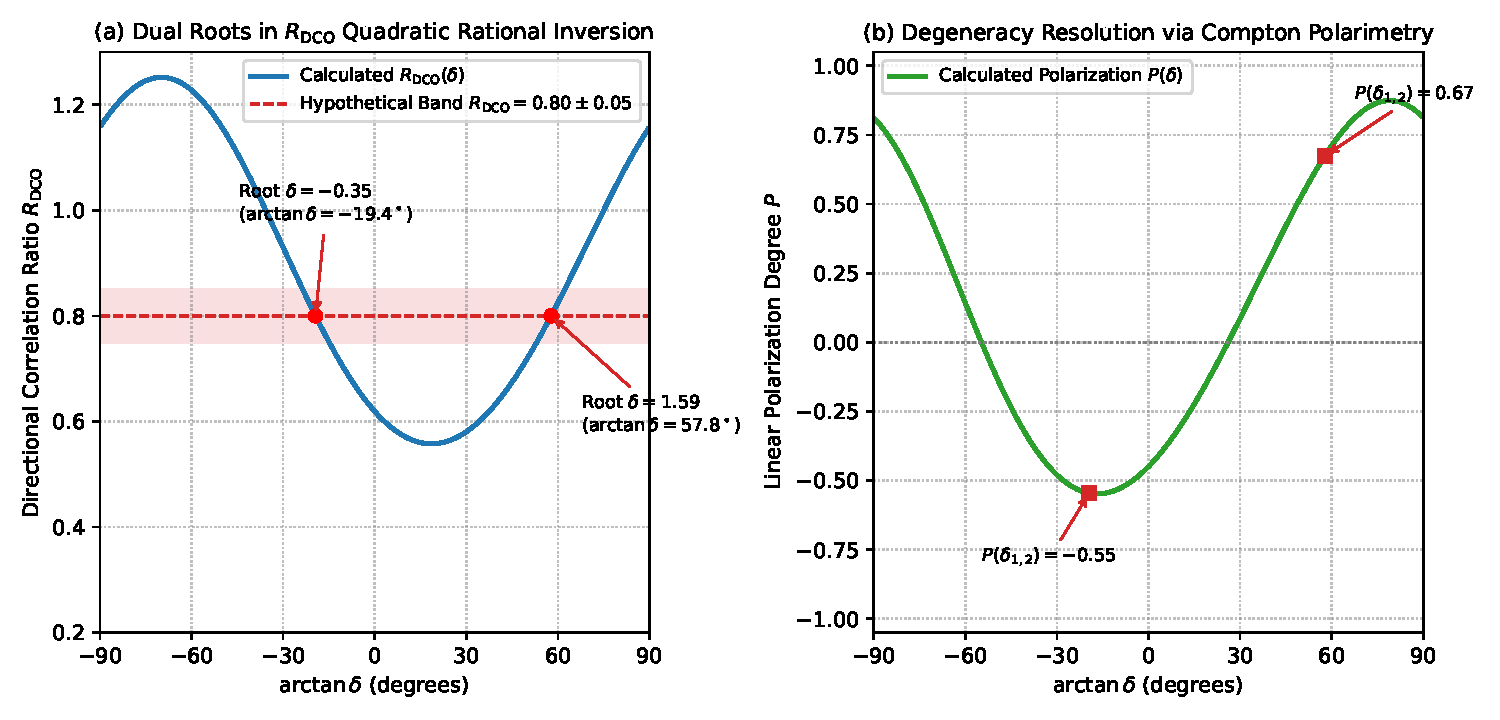
\includegraphics[width=0.92\textwidth]{Img/angular-branch-delta-likelihood.pdf}%
\caption[多极混合比 $\delta$ 的二次有理反演与偏振简并解除机制]{多极混合比 $\delta$ 的二次有理反演与偏振简并解除机制（规范教学模型）。(a) 展示由严格正定响应比值构造的 $R_{\mathrm{DCO}}(\delta)$ 关于 $\arctan\delta$ 的二次有理示意曲线（系数选取保证分子与分母在全实数域恒为正），水平阴影带代表假设观测带 $R_{\mathrm{DCO}} = 0.80 \pm 0.05$。假设带与曲线相交给出两个完全相容的数学根分支 $\delta_1 = -0.35$（$\arctan\delta_1 = -19.4^\circ$）与 $\delta_2 = +1.59$（$\arctan\delta_2 = +57.8^\circ$）；(b) 给出满足正交偏振强度非负条件（$W \pm H > 0$，即 $|P| < 1$ 恒成立）的示意线偏振度 $P(\delta)$ 理论曲线。在两个根位置偏振度呈现显著差异（在这组自选系数下，$P(\delta_1)\approx-0.55$、$P(\delta_2)\approx+0.67$；实际电磁归属仍须结合自旋序列和响应模型），直观说明仅靠 DCO 比值无法独立定解，在测量不确定度与探测灵敏度具备足够区分力时，可借助康普顿散射偏振计或内转换电子谱区分两支解；这些不同响应约束在统计上是否独立，仍须核对共同事件与校准。注意此处曲线为代数构造的自洽规范教学模型，用于阐释方法学原理，非特定核态或探测硬件的实测拟合。}
\label{fig:5-7-angular-branch}
\end{figure}

图~\ref{fig:5-7-angular-branch} 确立了低能核结构谱学分析的一条关键证据边界：
\begin{enumerate}
\item 独立实验数据的分支保留原则：
在仅有角分布或 DCO 比值测量、缺乏具有足够区分精度的偏振度或内转换系数数据时，\emph{应报告所有仍与数据相容的分离分支及各自误差}！
\item 理论模型偏好不得冒充独立实验判决：
在核结构理论比对中（例如轴对称刚性转子模型或三轴粒子-转子耦合模型），模型往往预言特定带间跃迁具有极小的 $\delta$ 或特定的四极主导性。研究人员绝不能为了迎合某种理论偏好，在实验报告中人为剔除另一个与数据相容的候选根。
\item 连续似然剖面（Likelihood Profile）构建：
在统计推断中，可通过构建轮廓似然比检验曲线 $-2\Delta\ln \max_{\boldsymbol{\eta}} \mathcal{L}(\delta, \boldsymbol{\eta}) + \text{const}$，其参考分布与置信度需按实际统计模型确定；满足渐近正则性时可采用相应的卡方标尺；若原始矩阵包含非泊松结构或系统协方差，而已发表观测矢量 $\mathbf{y}$、响应均值模型及协方差矩阵 $\mathbf{V}$ 足以支撑声明的误差近似，广义最小二乘仍可作为推断框架；它不自动保证非高斯、小样本或奇异协方差下的区间覆盖，需按实际模型处理约束并校准。由于 $\delta$ 在实数轴上可延伸至 $\pm \infty$，通常在有界坐标 $\theta_\delta \equiv \arctan\delta \in [-\pi/2, \pi/2]$ 上绘制全局拟合剖面，展示可能呈现的双极小值结构及其非对称置信区间，并将其作为后续第~5.10~节全篇测量模型整合的客观输入。
\end{enumerate}

以奇 $A$ 核 $^{163}\mathrm{Lu}$ 中三轴超形变摆动带（TSD）的研究为例（A. Görgen 等人 2004 年经典工作~\cite{campaign-g07-gorgen-2004-163lu-quadrupole-moments}），在反演 TSD2 向 TSD1 带间跃迁的绝对 $B(E2)_{\mathrm{out}}$ 与 $B(M1)_{\mathrm{out}}$ 几率时，作者直接借用了先前独立薄靶角关联与偏振实验测得的平均值 $\delta = -3.10^{+0.36}_{-0.44}$，并假定其在整个高自旋带保持稳定。必须澄清：该文自身并未在此厚靶高自旋测量中重新独立测定高自旋各态的偏振度，而是基于共享的先前实验输入；这一实例表明微观多极强度反演往往依赖于先验假定与外部辅助测量。

% 额外观测提供不同响应约束；统计独立性仍须核对共同事件与校准。
